\documentclass[a4paper]{report}
\usepackage[utf8]{inputenc}
\usepackage[portuguese]{babel}
\usepackage{hyperref}
\usepackage{a4wide}
\hypersetup{pdftitle={TP3:  Protocolo IP},
pdfauthor={João Teixeira, José Ferreira, Miguel Solino},
colorlinks=true,
urlcolor=blue,
linkcolor=black}
\usepackage{subcaption}
\usepackage[cache=false]{minted}
\usepackage{listings}
\usepackage{booktabs}
\usepackage{multirow}
\usepackage{appendix}
\usepackage{tikz}
\usepackage{authblk}
\usepackage{bashful}
\usepackage{verbatim}
\usepackage{amsmath}
\usetikzlibrary{positioning,automata,decorations.markings}
\AfterEndEnvironment{figure}{\noindent\ignorespaces}

\begin{document}

\title{TP4:\\ 
\large Grupo Nº 7}
\author{João Teixeira (A85504) \and José Ferreira (A83683) \and Miguel Solino (A86435)}

\date{\today}

\begin{center}
    \begin{minipage}{0.75\linewidth}
        \centering
        
\includegraphics[width=0.4\textwidth]{images/eng.jpeg}\par\vspace{1cm}
        \vspace{1cm}
        \href{https://www.uminho.pt/PT}
        {\color{black}{\scshape\LARGE Universidade do Minho}} \par
        \vspace{1cm}
        \href{https://www.di.uminho.pt/}
        {\color{black}{\scshape\Large Departamento de Informática}} \par
        \maketitle
    \end{minipage}
\end{center}

\tableofcontents

\chapter{3. Acesso Rádio}
\section{Exercício 1}
\textbf{Identifique em que frequência do espectro está a operar a rede sem fios,
e o canal que corresponde a essa frequência.}

\begin{figure}[H]
    \centering 
    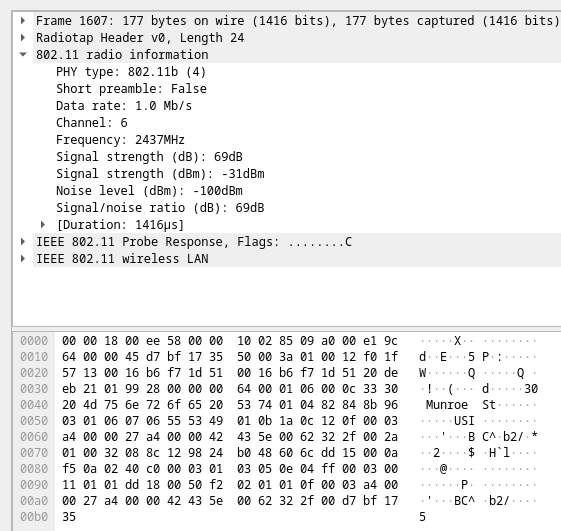
\includegraphics[width=\textwidth]{images/trama1607.png}  
    \caption{trama 1607}
    \label{fig:trama1607}
\end{figure}

\section{Exercício 2}
\textbf{Identifique a versão da norma IEEE 802.11 que está a ser usada.}

\section{Exercício 3}
\textbf{Qual o débito a que foi enviada a trama escolhida? Será que esse débito
    corresponde ao débito máximo a que a interface Wi-Fi pode operar?
    Justifique.}

\begin{figure}[H]
    \centering 
    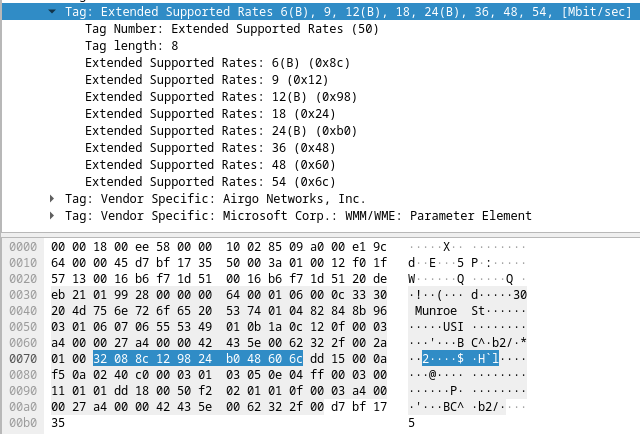
\includegraphics[width=\textwidth]{images/maxDataRate3.png}  
    \caption{Max Data Rate 3}
    \label{fig:maxDataRate3}
\end{figure}

\chapter{4. Scanning}
\section{Exercício 4}
\textbf{Quais são os SSIDs dos dois APs que estão a emitir a maioria das tramas
    de beacon?}
\begin{figure}[H]
    \centering 
    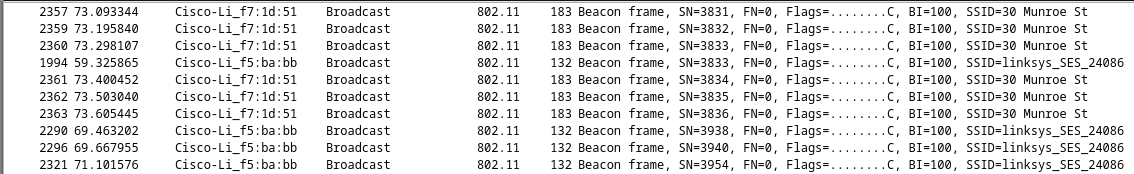
\includegraphics[width=\textwidth]{images/ex4SSIDS.png}  
    \caption{SSIDs}
    \label{fig:SSIDs}
\end{figure}

\section{Exercício 5}
\textbf{Qual o intervalo de tempo entre a transmissão de tramas beacon para o AP
    linksys\_ses\_24086? E do AP 30 Munroe St? (Pista: o intervalo está contido na
    própria trama). Na prática, a periodicidade de tramas beacon é verificada?
    Tente explicar porquê.}

\section{Exercício 6}
\textbf{Qual é (em notação hexadecimal) o endereço MAC de origem da trama beacon
    de 30 Munroe ST? Para detalhes sobre a estrutura das tramas 802.11, veja a
    secção 7 da norma IEEE 802.11 citada no início.}

\begin{figure}[H]
    \centering 
    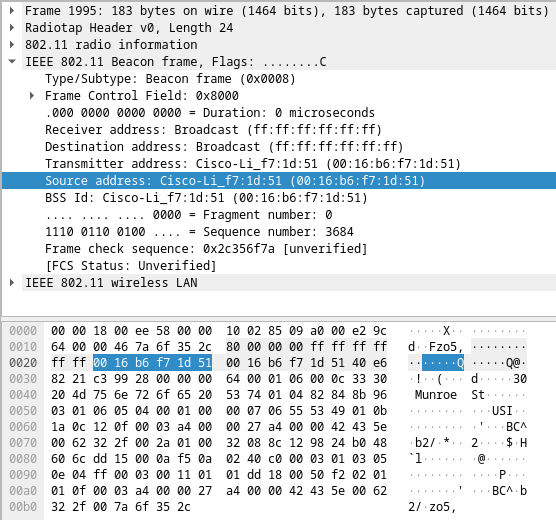
\includegraphics[width=\textwidth]{images/ex6.png}  
    \caption{Exercicio 6}
    \label{fig:ex6}
\end{figure}

\section{Exercício 7}
\textbf{Qual é (em notação hexadecimal) o endereço MAC de destino na trama de 30
    Munroe ST??}

\section{Exercício 8}
\textbf{Qual é (em notação hexadecimal) o MAC BSS ID da trama beacon de 20
    Munroe ST?}

\section{Exercício 9}
\textbf{As tramas beacon do AP 30 Munroe St anunciam que o AP suporta quatro
    data rates e oito extended supported rates adicionais. Quais são?}
\begin{figure}[H]
    \centering 
    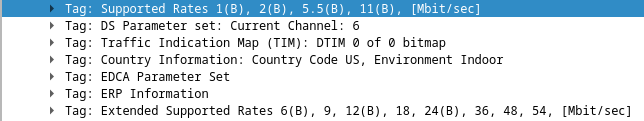
\includegraphics[width=\textwidth]{images/ex9.png}  
    \caption{Exercicio 9}
    \label{fig:ex9}
\end{figure}

\section{Exercício 10}
\textbf{Selecione uma trama beacon (e.g., a trama 1YXX com Y=turno e XX=grupo,
    e.g., 1101). Esta trama pertence a que tipo de tramas 802.11? Indique o
    valor dos seus identificadores de tipo e de subtipo. Em que parte concreta
    do cabeçalho da trama estão especificados (ver anexo)?}

\begin{figure}[H]
    \centering 
    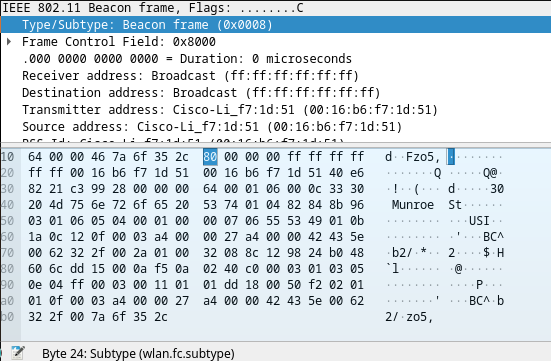
\includegraphics[width=\textwidth]{images/ex10.png}  
    \caption{Exercicio 10}
    \label{fig:ex10}
\end{figure}

\section{Exercício 11}
\textbf{Verifique se está a ser usado o método de deteção de erros CRC e se
    todas as tramas beacon são recebidas corretamente. Justifique o uso de
    mecaismos de deteção de erros neste tipo de redes locais.}

\begin{figure}[H]
    \centering 
    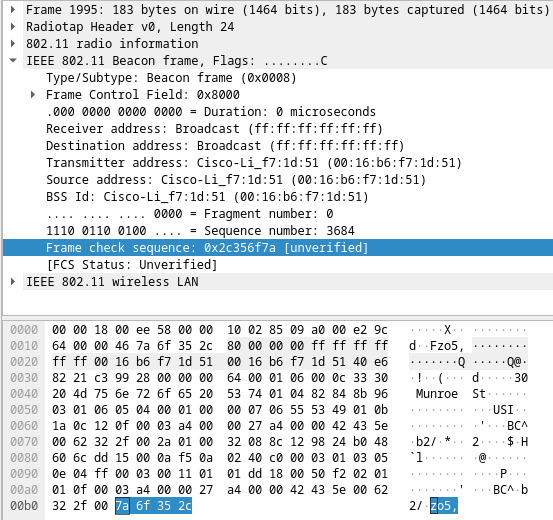
\includegraphics[width=\textwidth]{images/ex11.png}  
    \caption{Exercicio 11}
    \label{fig:ex11}
\end{figure}

\section{Exercício 12}
\textbf{Identifique e registe todos os endereços MAC usados nas tramas beacon
    enviadas pelos APs. Recorde que o endereçamento está definido no cabeçalho
    das tramas 802.11 podendo ser utilizados até quatro endereços com diferente
    semântica. Para uma descrição detalhada da estrutura da trama 802.11,
    consulte o anexo ao enunciado.}
\begin{figure}[H]
    \centering 
    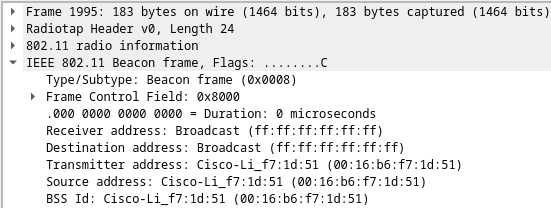
\includegraphics[width=\textwidth]{images/ex12p1.png}  
    \caption{Exercicio 12 - Parte 1}
    \label{fig:ex12p1}
\end{figure}

\begin{figure}[H]
    \centering 
    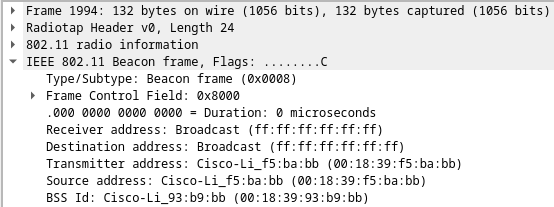
\includegraphics[width=\textwidth]{images/ex12p2.png}  
    \caption{Exercicio 12 - Parte 2}
    \label{fig:ex12p2}
\end{figure}

\section{Exercício 13}
\textbf{Estabeleça um filtro Wireshark apropriado que lhe permita visualizar
    todas as tramas probing request e probing response, simultaneamente.}

\begin{figure}[H]
    \centering 
    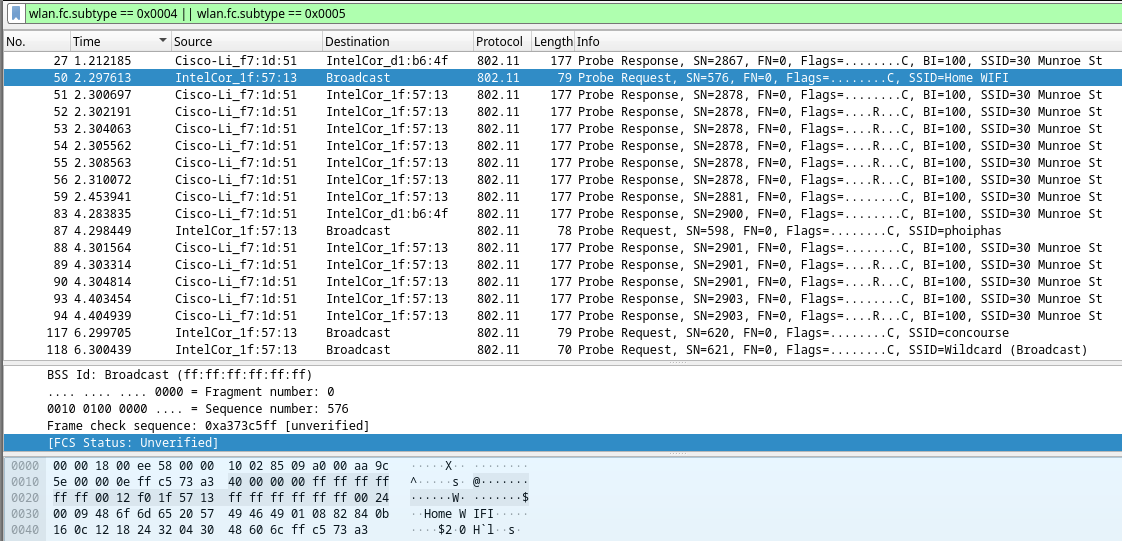
\includegraphics[width=\textwidth]{images/ex13.png}  
    \caption{Exercicio 13}
    \label{fig:ex13}
\end{figure}

\section{Exercício 14}
\textbf{Quais são os endereços MAC BSS ID de destino e origem nestas tramas?
    Qual o objetivo deste tipo de tramas?}

\section{Exercício 15}
\textbf{Identifique um probing request para o qual tenha havido um probing
    response. Face ao endereçamento usado, indique a que sistemas são
    endereçadas estas tramas e explique qual o propósito das mesmas?}

\chapter{6. Processo de Associação}
\section{Exercício 16}
\textbf{Quais as duas ações realizadas (i.e., tramas enviadas) pelo host no
    trace imediatamente após t=49 para terminar a ssociação com o AP 30 Munroe
    St que estava ativa quando o trace teve inicio= (Pista: uma é na camada IP e
    outra na camada de ligação 802.11). Observando a especificação 802.11, seria
    de esperar outra trama, mas que não aparece?}

\section{Exercício 17}
\textbf{Examine o trace e procure tramas de authentication enviadas do host para
    um AP e vice-versa. Quantas mensagens de authentication foram enviadas do
    host para o AP linkysys\_ses\_24086 (que tem o endereço MAC
    Cisco\_Li\_f5:ba:bb) aproximadamente ao t=49?}

\section{Exercício 18}
\textbf{Qual o tipo de autenticação pretendida pelo host, aberta ou usando uma
    chave?}

\section{Exercício 19}
\textbf{Observa-se a resposta de authentication do AP linksys\_ses\_24086 AP no
    trace?}

\section{Exercício 20}
\textbf{Vamos agora considerar o que acontece quando o host desiste de se
    associar ao AP linksys\_ses\_24086 AP e se tenta associar ao AP 30 Munroe
    St. Procure tramas authentication enviadas pelo host para e do AP e
    vice-versa. Em que tempo aparece um trama authentication do host para o AP
    30 Munroe St. e quando aparece a resposta authentication do AP para o host?}

\section{Exercício 21}
\textbf{Um associate request do host para o AP e uma trama de associate response
    correspondente do AP para o host são usados para que o host seja associado a
    um AP. Quando aparece o associate request do host para o AP 30 Munroe St?
    Quando é enviado o correspondente associate reply?}

\section{Exercício 22}
\textbf{Que taxas de trasmissão o host está disposto a usar? E o AP?}

\section{Exercício 23}
\textbf{Identifique uma sequência de tramas que corresponda a um processo de
    associação completo entre a STA e o AP, incluindo a fase de autenticação.}

\chapter{7. Transferência de Dados}
\section{Exercício 24}
\textbf{Efetue um diagrama que ilustre a sequência de todas as tramas trocadas
    no processo de associação, incluindo a fase de autenticação}

\section{Exercício 25}
\textbf{Encontre a trama 802.11 que contém o segmento SYN TCP para a primeira
    sessão TCP (download alice.txt). Quais sao os três campos do endereços MAC
    na trama 802.11?}

\section{Exercício 26}
\textbf{Qual o endereço MAC nesta trama que corresponde ao host (em notação
    hexadecimal)? Qual o do AP? Qual o do router do primeiro salto? Qual o
    endereço IP do host que está a enviar este segmento TCP? Qual o endereço IP
    de destino?}

\section{Exercício 27}
\textbf{Este endereço IP de destino corresponde ao host, AP, router do primeiro
    salto, ou outro equipamento de rede? Justifique.}

\section{Exercício 28}
\textbf{Encontre agora a trama 802.11 que contém o segmento SYNACK para esta
    sessão TCP. Quais são os três campos dos endereços MAC na trama 802.11?}

\section{Exercício 29}
\textbf{Qual o endereço MAC nesta trama que corresponde ao host? Qual o do AP?
    Qual o do router do primeiro salto?}

\section{Exercício 30}
\textbf{O endereço MAC de origem na trama corresonde ao endereço IP do
    dispositivo que enviou o segmento TCP encapsulado neste datagrama?
    Justifique.}

\chapter{Conclusão}
A realização deste trabalho proporcionou nos a oportunidade de aprofundar os
nossos conhecimentos relativamente a Ethernet, Endereços MAC, Address Resolution
Protocol (ARP) e Interligação de Redes Locais.\\
Utilizando a ferramenta Wireshark e o Core conseguimos capturar e analisar
tramas Ethernet, ou seja, o essencial para colocarmos em prática e aprimorar os
nossos conhecimentos relacionados com os tópicos anteriormente referidos.\\
Se dividirmos o trabalho por partes é possível dividir em 3. Na primeira parte o
foco foi baseado na utilização de uma conexão por Ethernet. Na segunda foi
focado nos pacotes ARP e na terceira a comparação entre Hubs e Switches.
Resumindo, achamos que maior parte do capitulo Link Layer foi abrangido e
relembrado.

\end{document}
